


\subsection{Training Data Generation}

The finite element models were designed to be as consistent as possible with the work presented in \cite{RNeqnsbook}, while using modern computational tools. Using similar boundary conditions (BCs) allows for the comparison between GPSR and the equations created in \cite{RNeqnsbook}. The cracked finite element models are entirely defined by the variables $a$, $c$, $b$, $t$, $h$, and $u$ shown in figure \ref{fig:model_params}. The far field stress $\sigma$ is extracted from the reaction forces at the top and bottom surfaces. The variables $a$ and $c$ are crack parameters and the variables $b$, $t$, and $h$ define the geometry of the plate.

\begin{figure}%
    \centering
    \subfloat[\centering Applied boundary conditions]{{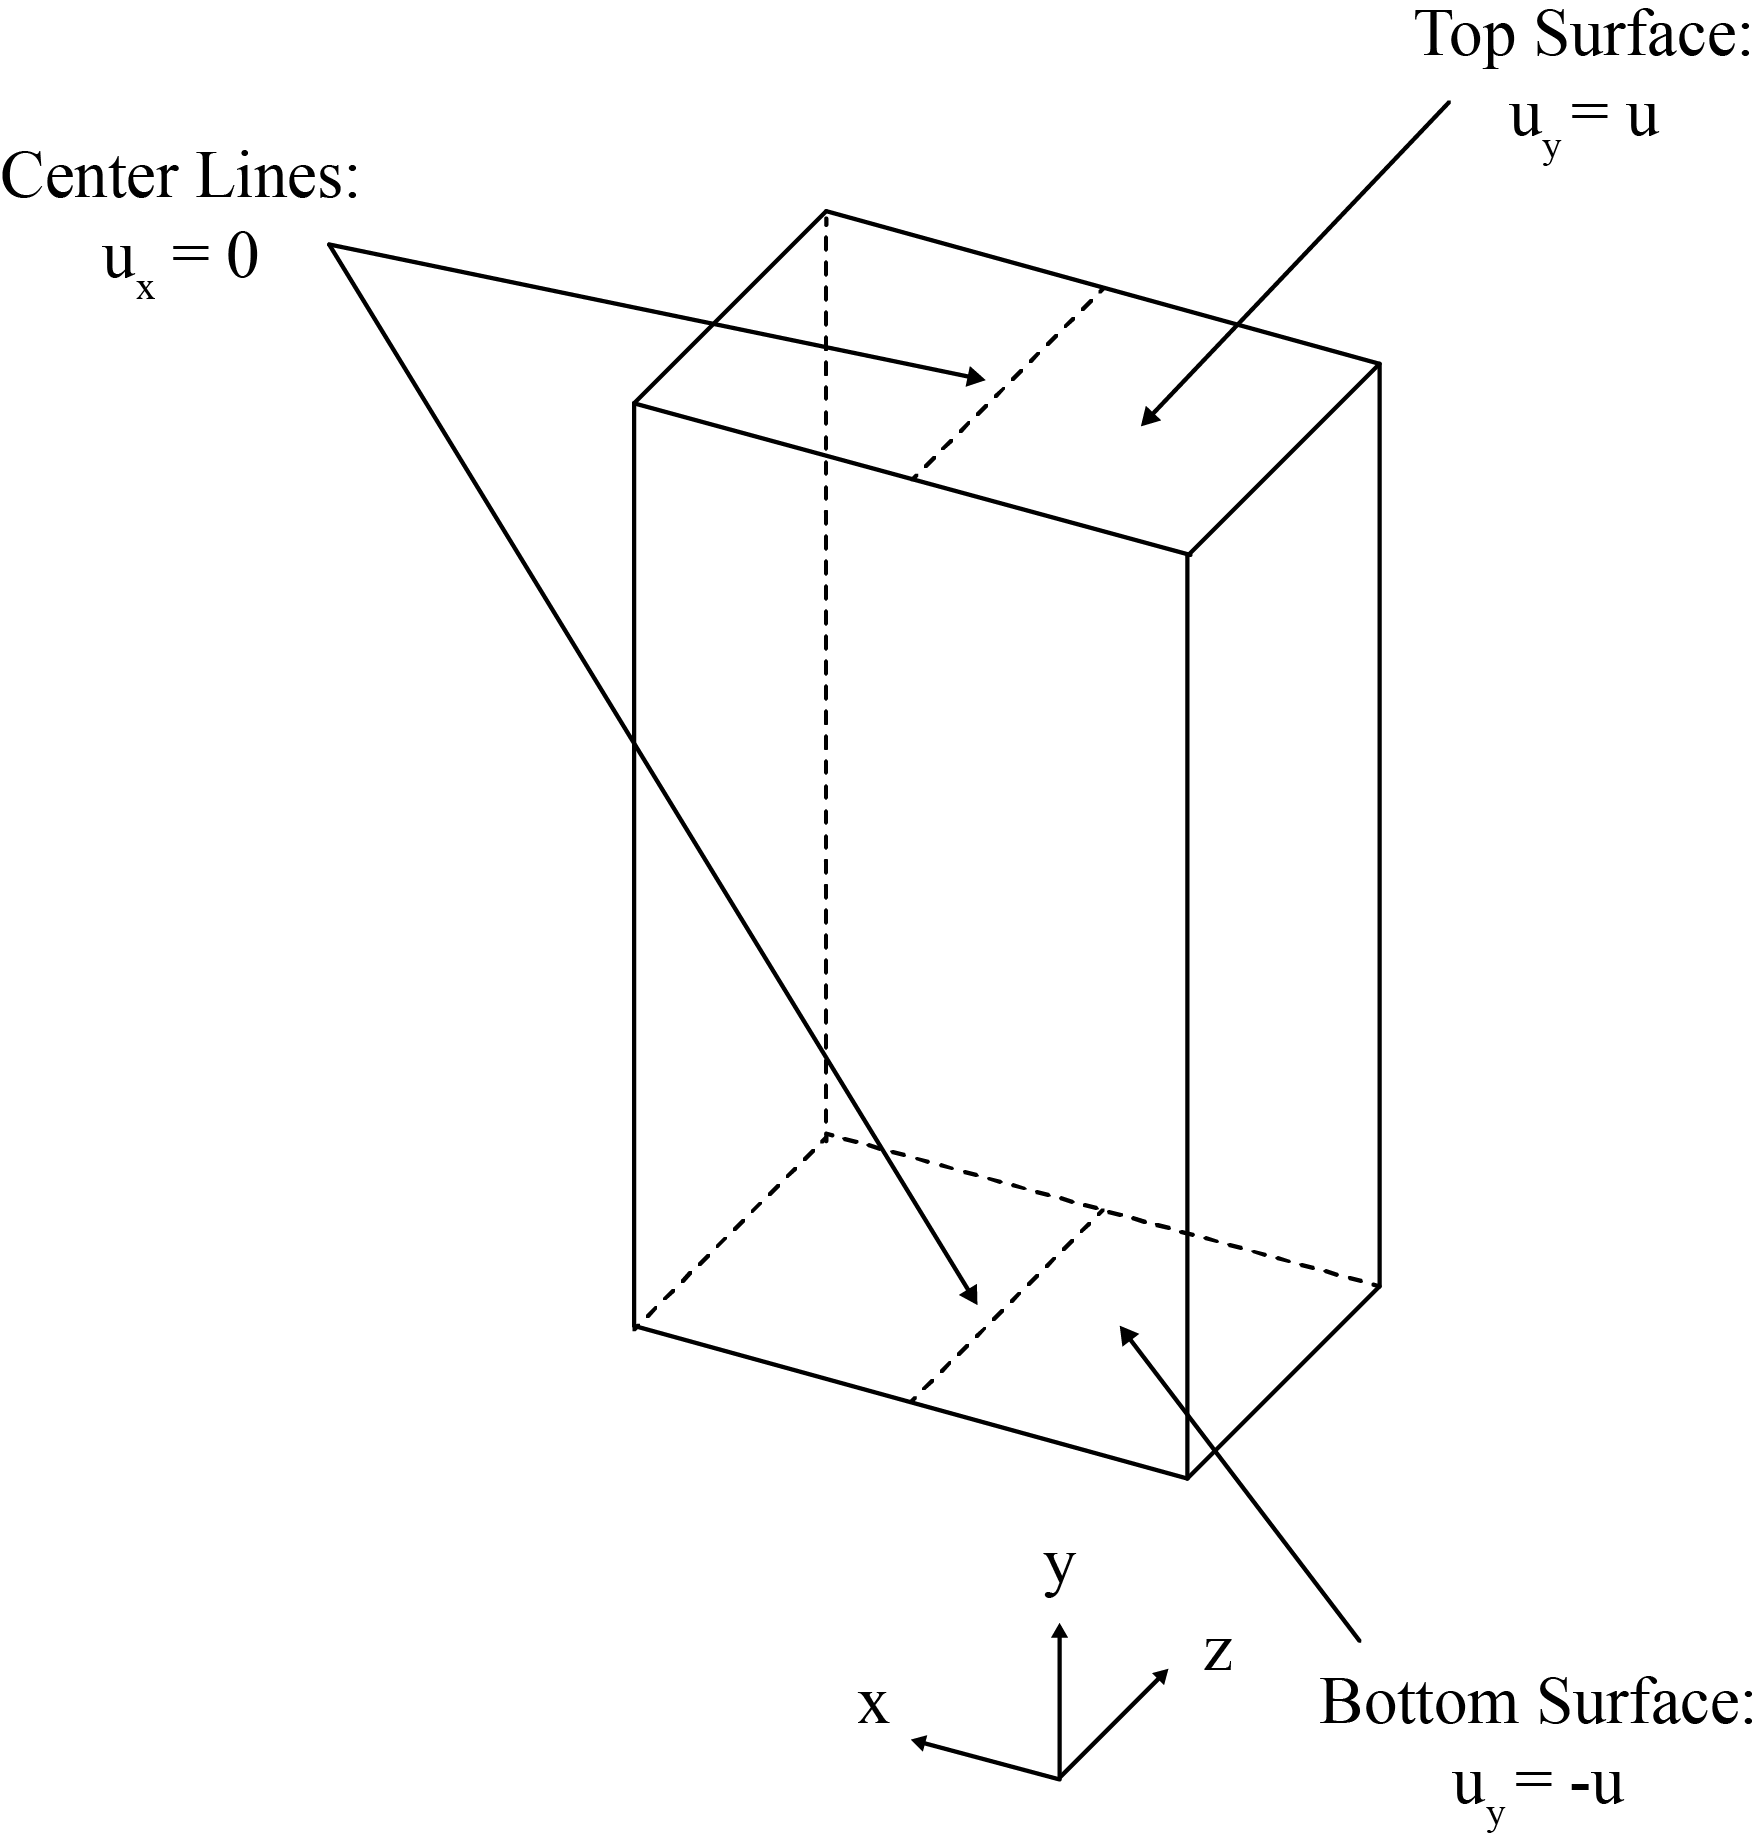
\includegraphics[width=0.6\textwidth]{geometry_figures/BCs.png} }}%
    \qquad
    \subfloat[\centering Model geometry]{{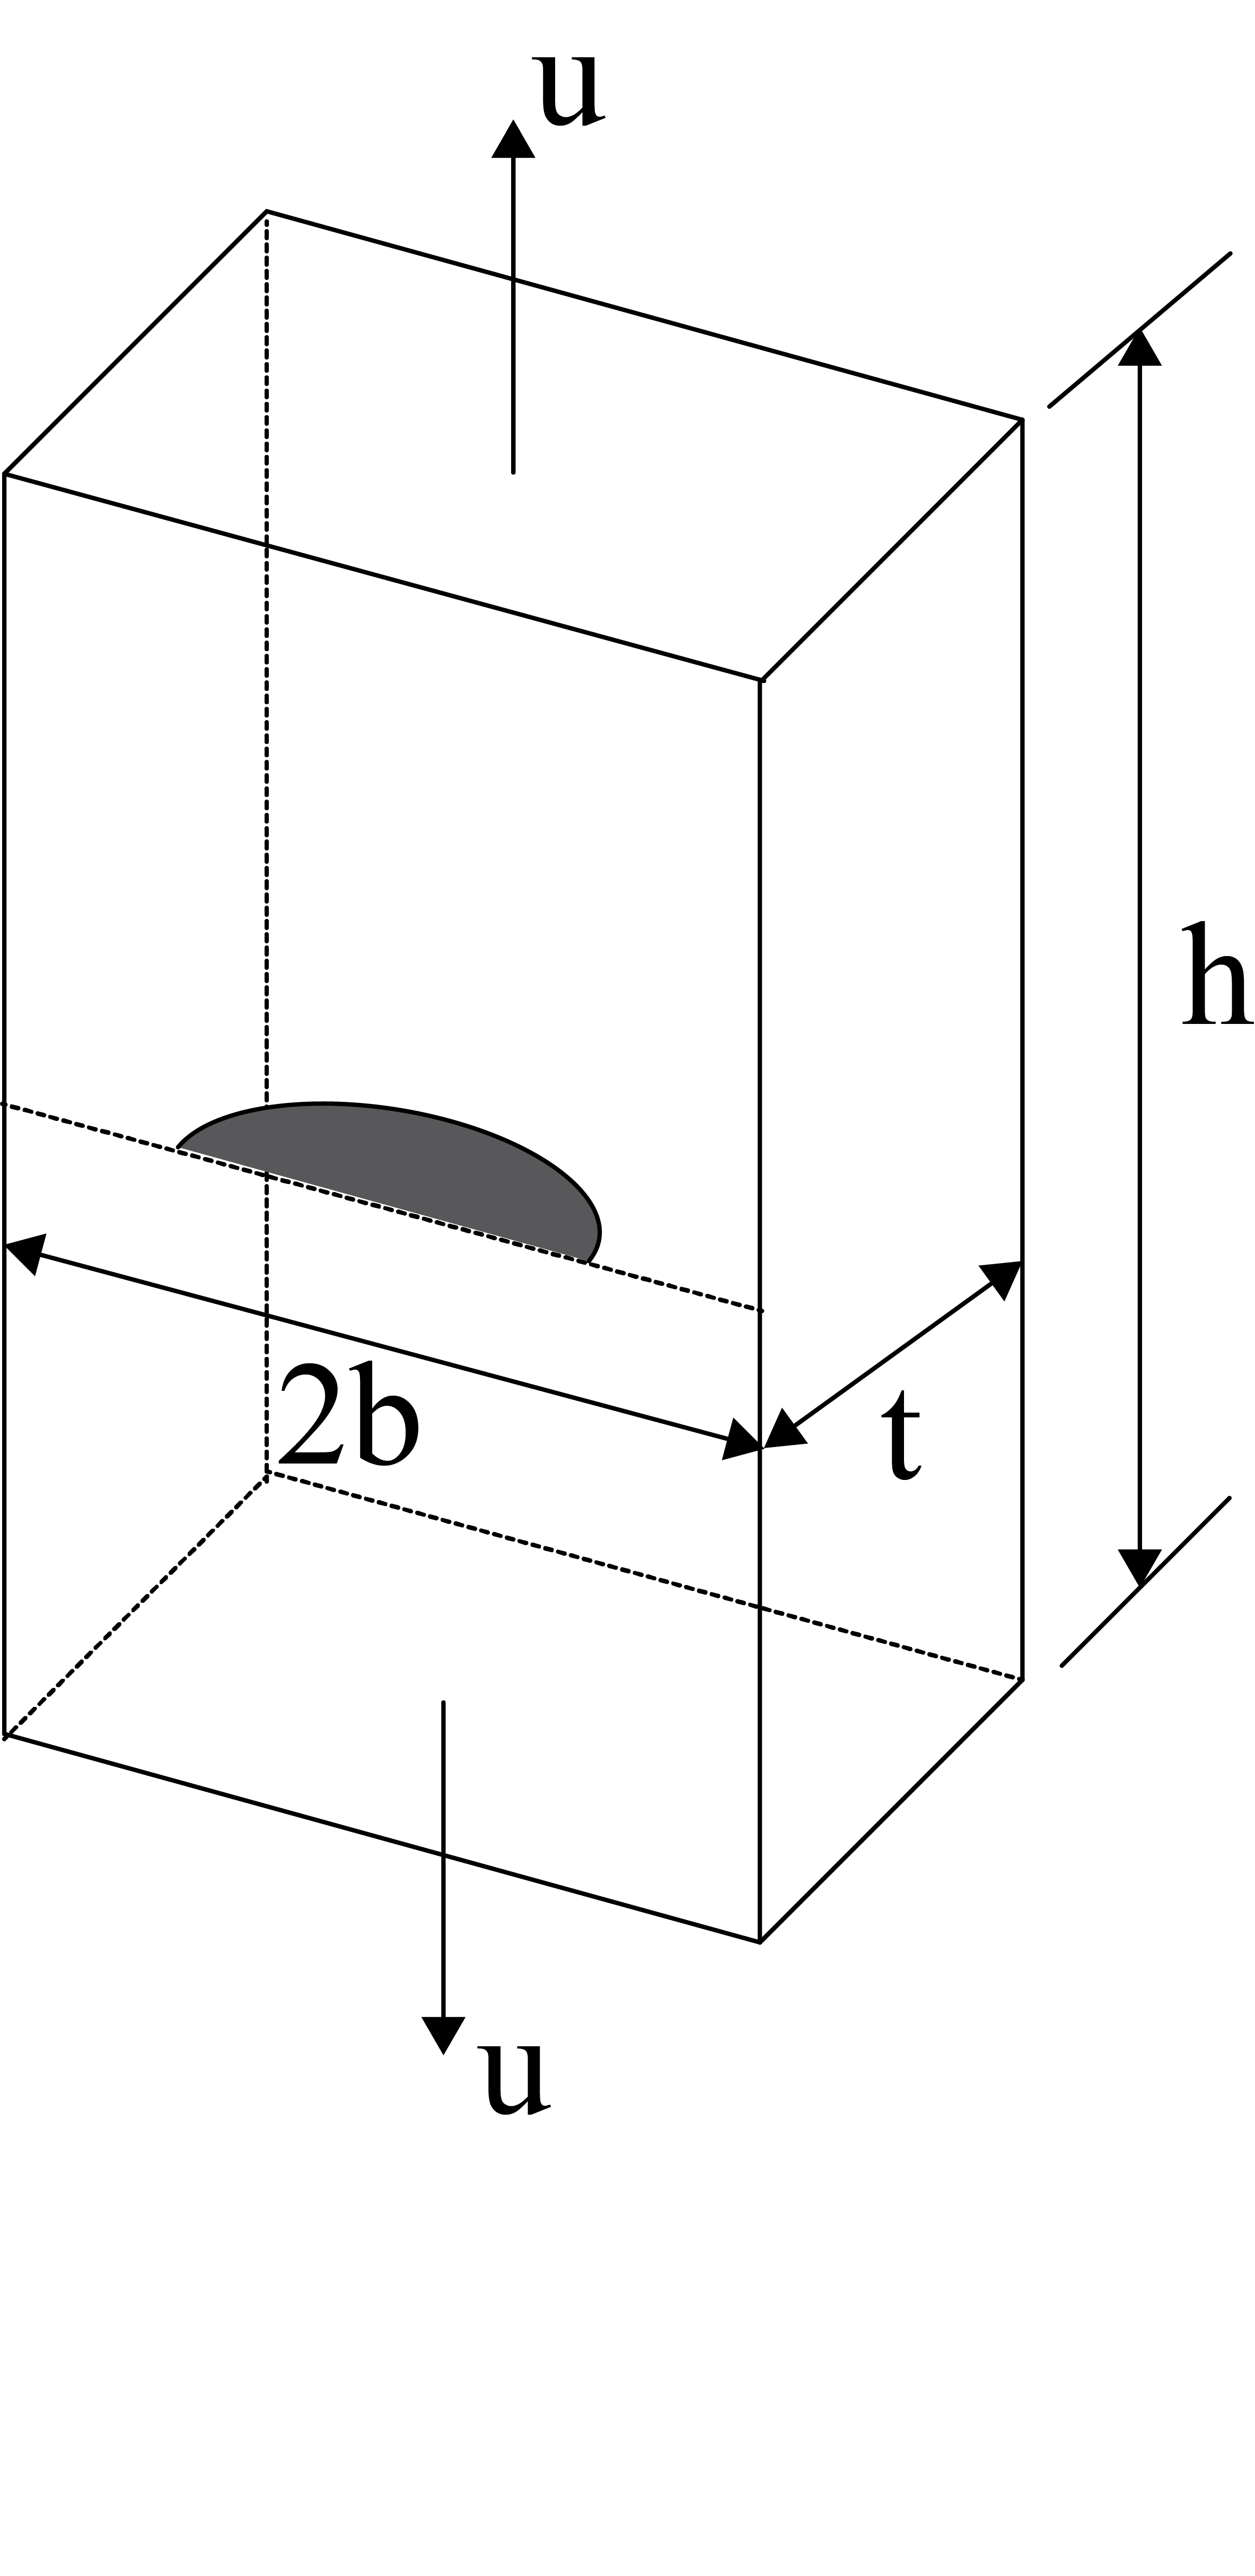
\includegraphics[width=0.3\textwidth]{geometry_figures/Geom.png} }}%
    \caption{(a) Top and bottom surfaces with displacement in $+y$ and $-y$ respectively. The center lines of the top and bottom faces are held $0$ in $x$. (b) Model geometry plate hight: $h$, plate width: $2b$, and plate thickness: $t$.}%
    \label{fig:model_params}%
\end{figure}
	
%uncracked model
In \cite{RNeqnsbook}, Raju and Newman neglected effects due to finite height by assuming the height of the plate to be large relative to the thickness of the plate. To be consistent with this assumption, a constant value of $h/t = 64$ was chosen to remove any effects due to the height of the plate as shown in figure \ref{fig:h_convergence}. As stated previously the BCs of the models were made to match the models from \cite{RNeqnsbook} without overly constraining the model as depicted in figure \ref{fig:model_params}. A constant displacement of $u = 0.001$ units was applied on the top and bottom surfaces in the direction of the surface normals. Additionally the center-lines of the top and bottom surfaces were held fixed in the x-direction to removed rigid body motion. 
\begin{figure}
    \centering
    \subfloat[\centering Convergence of $h/t$]{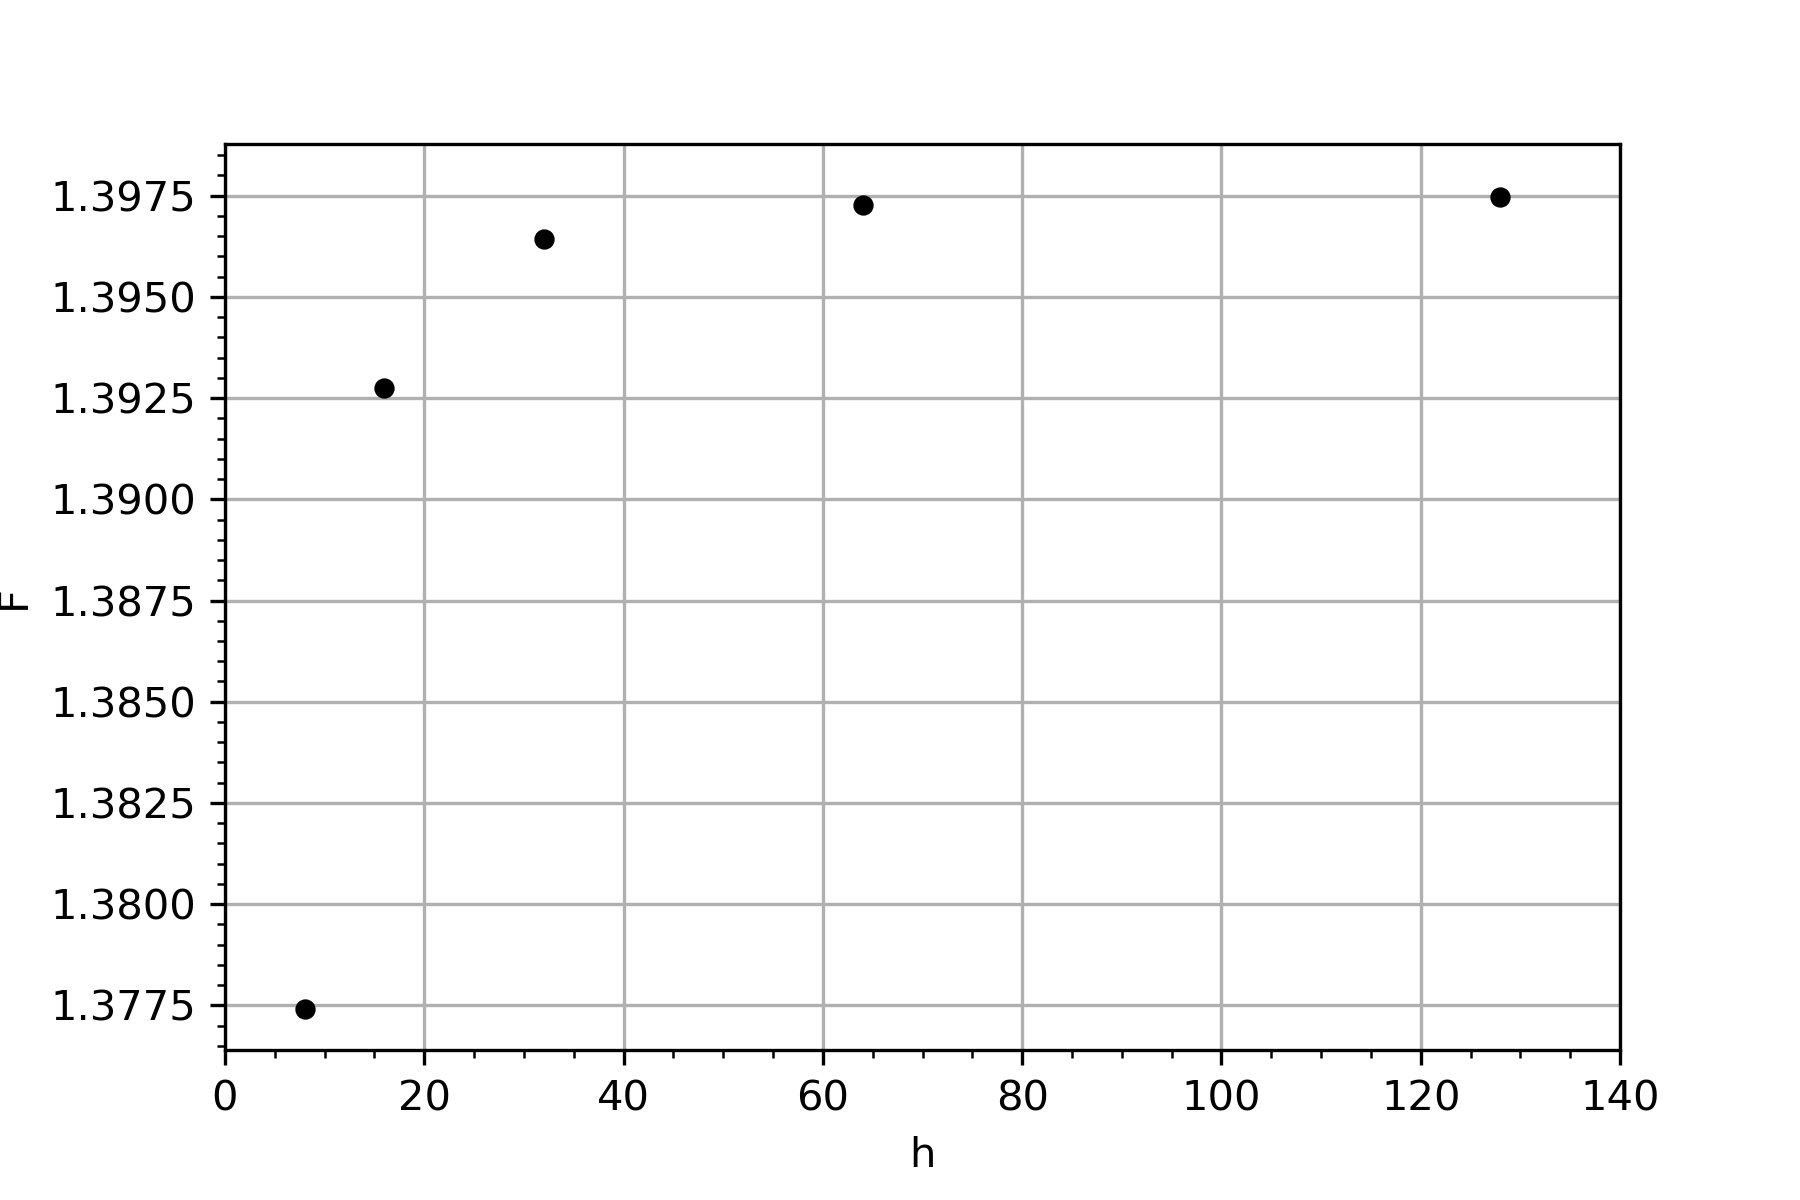
\includegraphics[width=0.45\textwidth]{Figures/h_convergence.png}\label{fig:h_convergence}}%
    \qquad
    \subfloat[\centering Convergence of $c/b$]{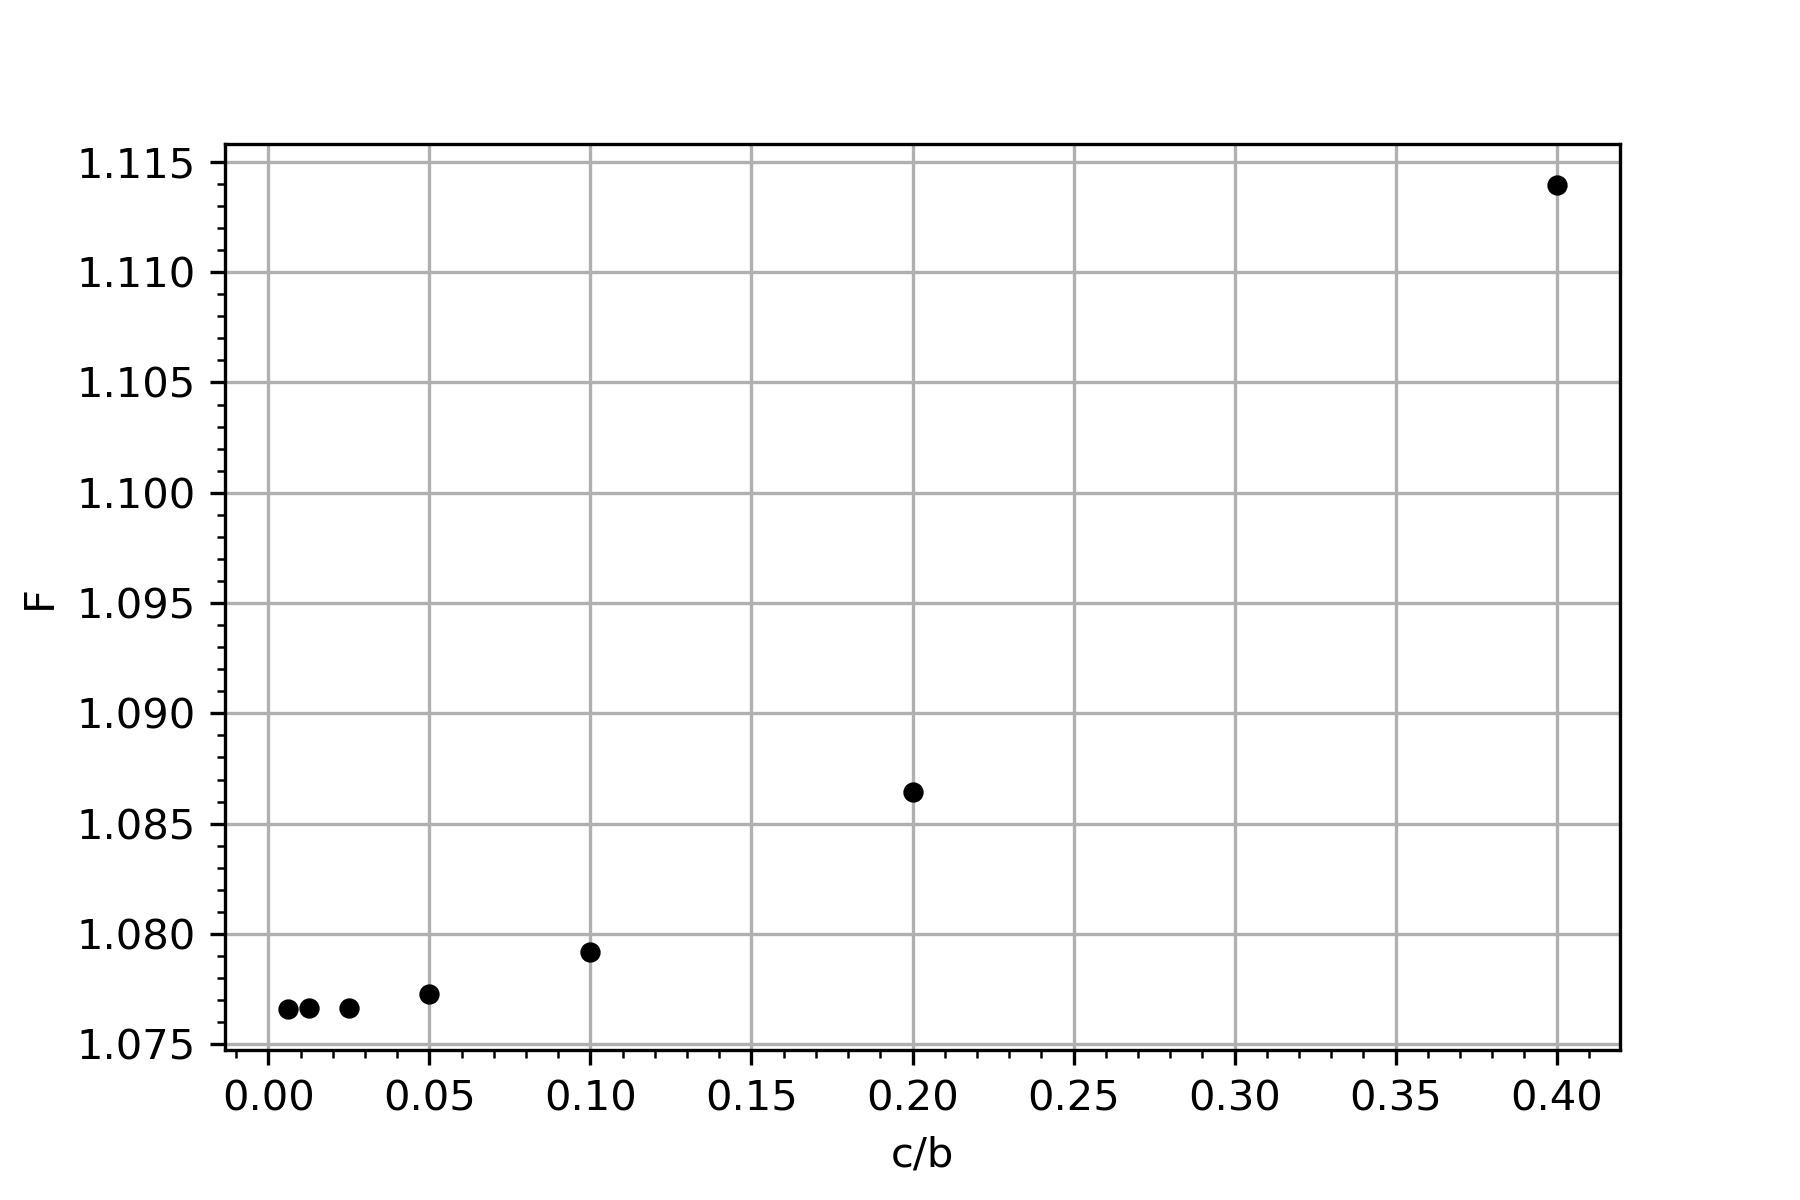
\includegraphics[width=0.45\textwidth]{Figures/cb_convergence.png}\label{fig:cb_convergence}}
    \caption{(a) The convergence of $h/t$ is plotted using the mean boundary correction factor. (b) The convergence of $c/b$ is plotted using the mean boundary correction factor.}
    \label{fig:convergence_plots}
\end{figure}

\begin{table}[]
\centering
\begin{tabular}{|l|l|l|l|}
\hline
\textbf{Feature} & \textbf{min} & \textbf{step} & \textbf{max} \\ \hline
a/c              & 0.2          & 0.05          & 2            \\ \hline
a/t              & 0.2          & 0.05          & 0.8          \\ \hline
c/b              & 0.01         & 0.05          & 0.4          \\ \hline
$\phi$           & 0            & $\pi / 150$  & $\pi$        \\ \hline
\end{tabular}
\caption{Max and min values for each of the features used when creating the cracked FE models}
\label{table:feat_range}
\end{table}


The crack mesh created by FRANC3D is shown in \ref{fig:f3d_crack}. The mesh contains a ring of quarter points elements around the crack front followed by rings of brick elements. The parameters for the crack mesh are the template radius which specifies the size of each element; the number of rings of elements around the crack; and the number of circumferential elements in each ring. Instead of using a fixed template radius a number of elements along the entire crack was specified. This produced better results with varying crack aspect ratios. The best SIF values were computed with 300-600 elements along the crack, 8 rings of elements, and 14 circumferential elements per ring as shown in table \ref{table:optimized_vals}. The average SIF value for each model is relatively insensitive to the crack mesh, however certain crack geometries display numerical noise for certain crack mesh sizes as shown in figure \ref{fig:crack_mesh_convergence}. The models that displayed the most numerical noise for the most crack sizes were the models with values close to the following: $a/c = 0.5$, $a/t = 0.6$, and $c/b = 0.2$. The crack mesh parameters were chosen based off of these models and then applied to the rest of the models. Before running the entire data-set, a random sample of 10\% of the total models was computed to check for convergence. After convergence was confirmed on those models the entire data-set was computed. 

\begin{figure}
    \centering
    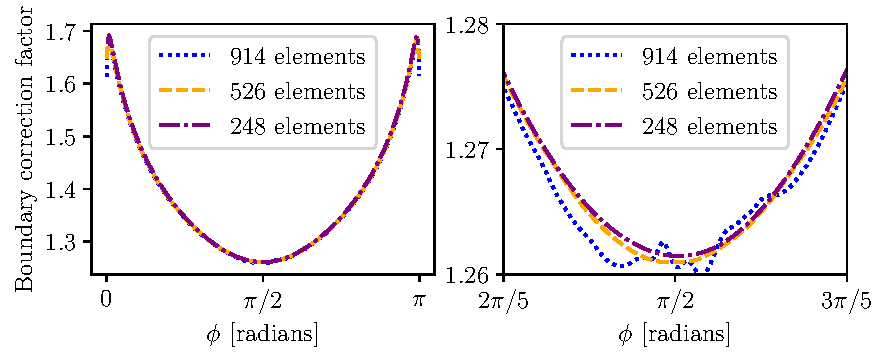
\includegraphics[width=\textwidth]{Figures_pdf/numerical_noise.pdf}
    \label{fig:crack_mesh_convergence}
    \caption{(left) entire SIF plot for differing number of elements along the crack front. (right) plot zoomed in at $\pi/2$ to highlight numerical noise with high element count.}
\end{figure}



The converged values are tabulated in table \ref{table:optimized_vals}
\begin{table}[]
\centering
\begin{tabular}{|l|l|}
\hline
Thickness                   & 1         \\ \hline
h/t                         & 64        \\ \hline
Global seed                 & max(0.25, min(b/50, 0.5))      \\ \hline
Local seed                  & 0.25      \\ \hline
Number of rings             & 8         \\ \hline
Number of circumferential elements             & 14        \\ \hline
Number crack front elements & $\sim$300 \\ \hline
\end{tabular}
\caption{Optimized model and mesh values}
\label{table:optimized_vals}
\end{table}




After the converged model parameters were found all 2500 of the models were run to calculate 300-450 SIFs per model. Figure \ref{fig:selected_sifs} shows the calculated SIF values from a few of the models compared to the SIFs calculated from \cite{RNFEM}.  

\begin{figure}
    \centering
    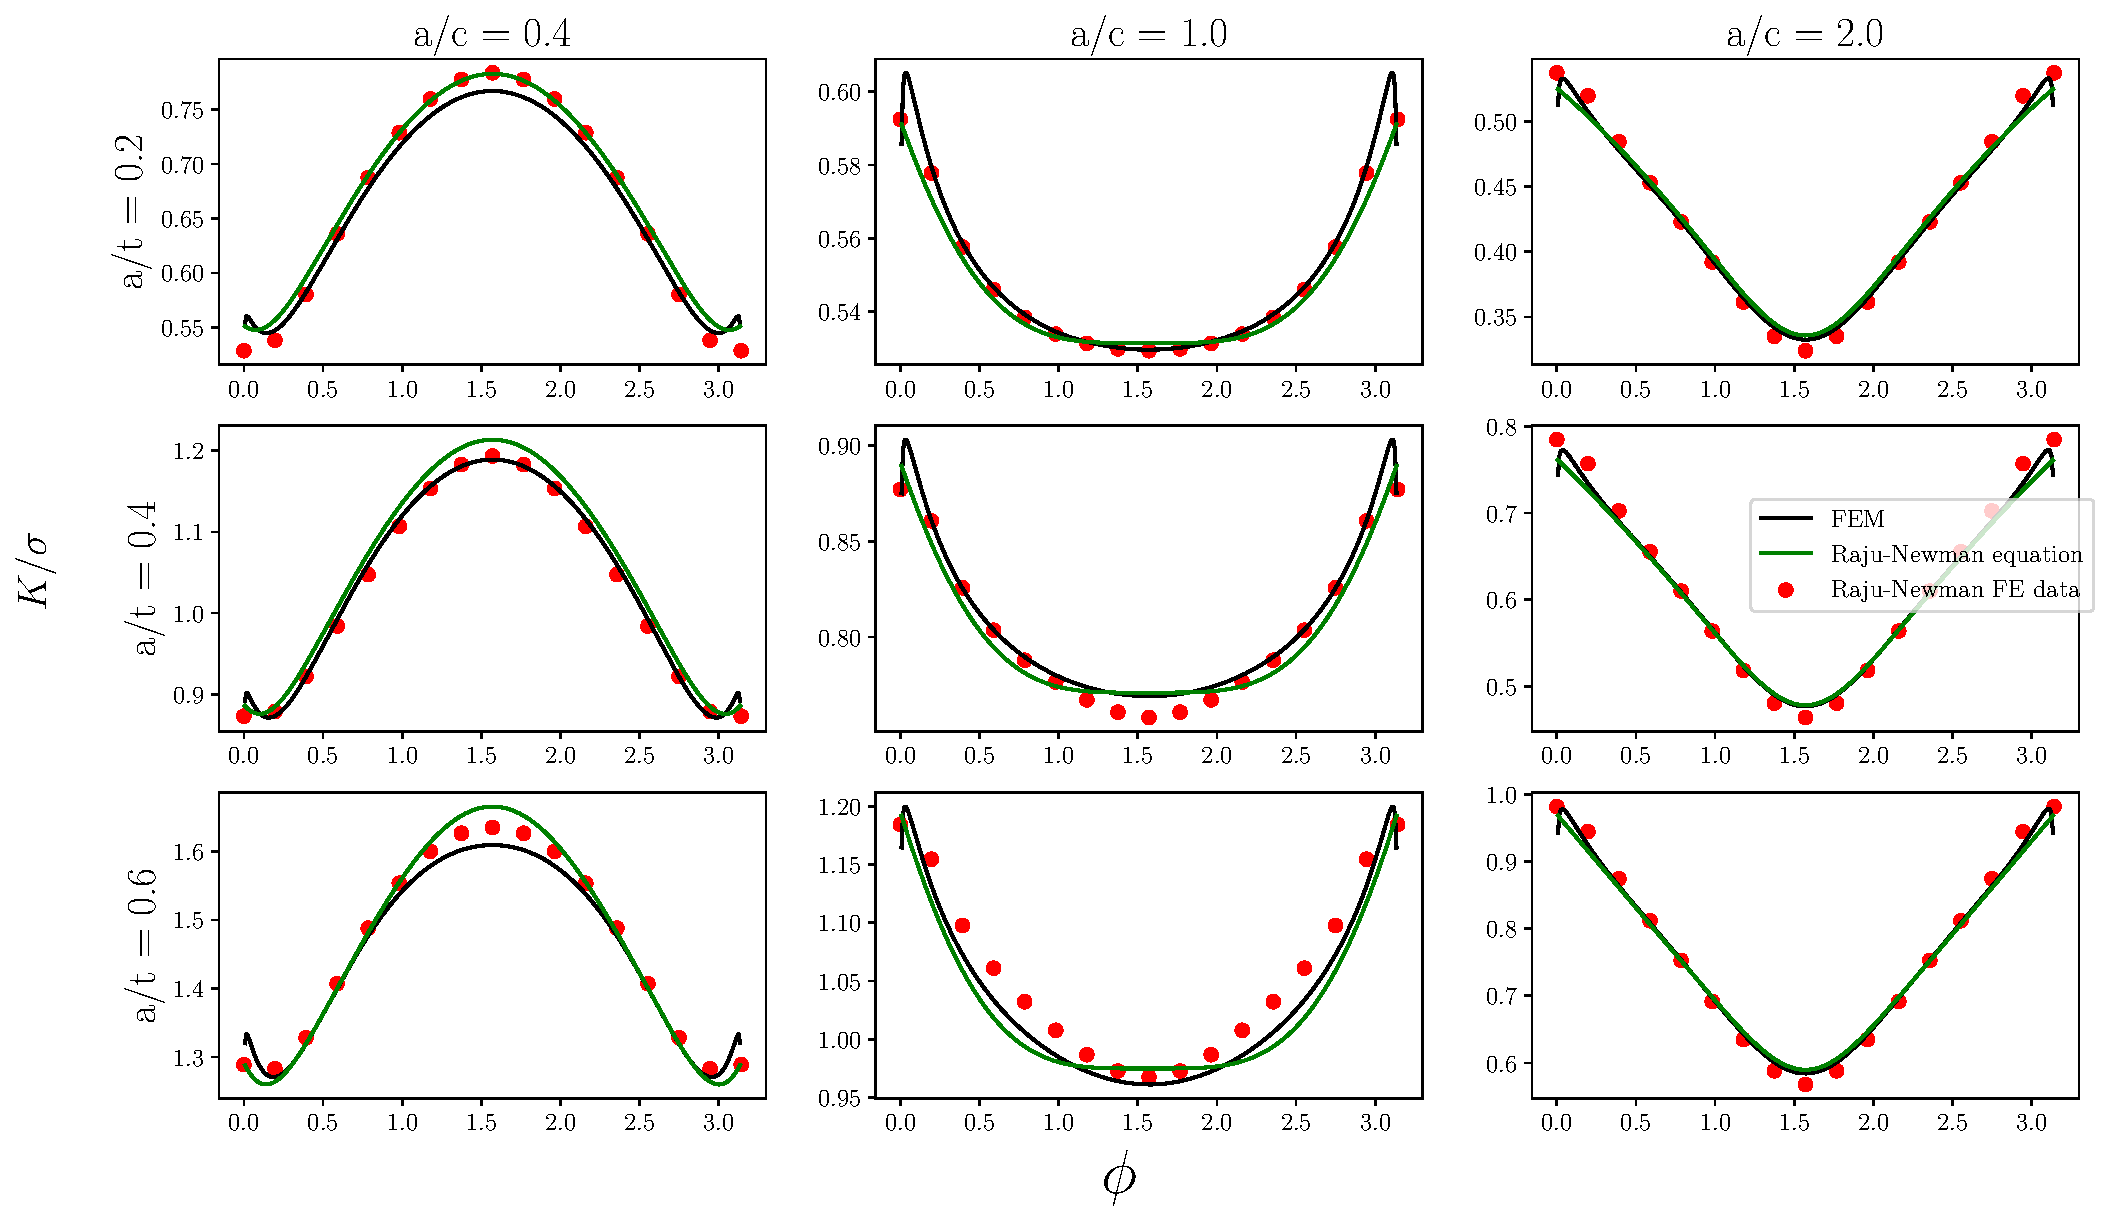
\includegraphics[width=\textwidth]{Figures_pdf/K_data.pdf}
    \label{fig:selected_sifs}
    \caption{SIF values from a selection of models plotted with the Raju-Newman equation.}
\end{figure}

%%%%%%%%%%%%%%%%%%%

\subsection{Training Data Subdivision}

The 2500 models were used for training and model selection, While a additional isolated set of 400 models were generated for testing to allow for better generalization error predictions. Instead of directly training on the SIF data extracted from FRANC3D this paper uses a mechanics based approach to simplify the training process which increases the explainablity of the final SIF model. The approach used in \cite{RNeqnsbook} was used to break the model for $K$ into two parts: the known part and the learned part. The known part includes equation \ref{eqn:K_embedded_ellipse}, which is the solution to the embedded ellipse in an infinite volume. The learned part of the equation is the boundary correction factor which is comprised of three sub-functions $f_w$, $M$, and $g$ each accounting for a different deviation from the infinite case. The finite width correction factor $f_w$ accounts for the effect of finite width and thickness at the center of a semi-circular crack. The $M$ equation expands on $f_w$ by accounting for the aspect ratio of the crack. The two functions $f_w$ and $M$ together comprise the boundary correction factor for the center of a semi-elliptical crack in a finite plate. Finally the $g$ equations takes this correction at the center and applies it to the rest of the crack allowing for SIFs to be predicted along the entire length of the crack. GPSR is especially suited for this process as it finds closed form equations which can conform exactly to the known limits of each of the boundary correction terms significantly increasing interpretability.

Two modifications were made to the approach used in \cite{RNeqnsbook} to make the training process easier and the resulting models more interpretable. The first is the method to modify the embedded ellipse equation to allow for $a/c > 1$. This was done by using the function $l$ from \cite{tada1985} and modifying it to allow for  $a/c > 1$ as shown in equation \ref{eqn:l}


\begin{equation} \label{eqn:l}
l = a \left( \frac{c}{\alpha} \right)^2 \sqrt{\left( \frac{a}{c} \right)^2 \cos^2 \phi + \sin^2 \phi},
\end{equation}

where $a$ is the crack depth, $c$ is half-crack surface length, and $\alpha$ is the length of the major axis of the ellipse. The function $l$ is a sort of pseudo radius which is a measure of the perpendicular distance from the tangent line at the point of interest to the nearest axis seen in figure \ref{fig:crack_params}. The benefit of modifying the embedded ellipse equation by using equation \ref{eqn:l} is that it removes the need for any piece-wise functions (like those use in \cite{RNeqnsbook}), as the that is all handled by the variable $\alpha$. This reduces the number of models that have to be trained from five as in \cite{RNeqnsbook} to three, one for each of $f_w$, $M$, and $g$. This reduces training time and lowers the complexity of the final $K$ solution resulting in a more interpretable equation. 

The second modification is the formulation of $f_w$, while Raju and Newman used a 3D modification of a finite width correction factor for a 3d through crack from \cite{brown1966}, this work will create a finite width correction factor specifically for the case of a semi-elliptical surface crack. To be able to use the process outlined in \cite{RNeqnsbook} The $f_w$ function was created as similarly as possible to the one use by Raju and Newman in order to be able to use their method of breaking down the equation. This means that $f_w$ will still be a finite width and thickness correction when $\phi = \pi/2$ and $a/c = 1$. 

When $\phi = \pi/2$ and $a/c = 1$ the value of $K$ converges to the embedded ellipse equation as $a/t$ and $c/b$ go to zero as seen in figure \ref{fig:fw_convergence}. This results in $f_w$ being defined as equation \ref{eqn:fw_parameter_def}

\begin{figure}
    \centering
    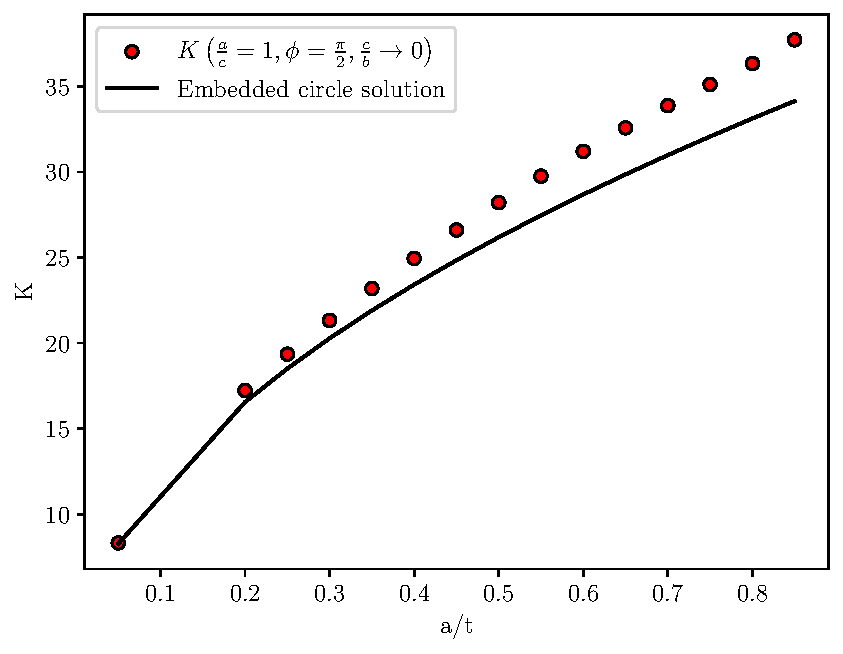
\includegraphics[width=\textwidth]{Figures_pdf/fw_convergence.pdf}
    \label{fig:fw_convergence}
    \caption{Comparison of K from the center of a surface crack and the solution to an embedded circle crack in an infinite volume as a function of a/t where c/b = 0.01, which has been determined to be close to 0 \ref{fig:convergence_plots}}
\end{figure}


\begin{equation} \label{eqn:fw_parameter_def}
    f_w\left(\frac{c}{b}, \frac{a}{t}\right) = \frac{K\left(\frac{a}{c} = 1, \phi = \frac{\pi}{2}\right)}{\sigma \frac{2}{\pi} \sqrt{\pi a}},
\end{equation}

resulting in $f_w$ correcting for finite width and thickness effects. The final equation for $K$ will be in the form of equation \ref{eqn:K_semi_with_l} 

\begin{equation} \label{eqn:K_semi_with_l}
    K = \sigma \frac{\sqrt{\pi l}}{E} f_w M g,
\end{equation}

where $f_w$, $M$, and $g$ are the boundary correction functions learned by Bingo and $\sigma \sqrt{\pi l}/E$ is the modified embedded ellipse solution. 


The process of extracting the training data from the SIF data calculated from the FE models is outlined here.
\begin{equation} \label{eqn:K_parameter_def}
    K\left(\frac{a}{c}, \frac{a}{t}, \frac{c}{b}, \phi, \sigma \right) = K_{ee} \left(
\frac{a}{c}, \sigma, \phi \right) f_w \left(\frac{a}{t}, \frac{c}{b} \right) M \left(\frac{a}{t}, \frac{a}{c} \right) g \left(\frac{a}{t}, \frac{a}{c}, \phi \right)
\end{equation}

The process of calculating the $f_w$ training data was previously shown in equation \ref{eqn:fw_parameter_def}. The next step is to extract the training data for $M$, which is computed similarly to $f_w$. The SIF data from FEA data is taken at $c/b = 0$ and $\phi = \pi/2$ then divided by equation \ref{eqn:K_embedded_ellipse} and equation \ref{eqn:fw_parameter_def} evaluated at $\phi = \pi/2$ resulting equation \ref{eqn:M_parameter_def} that is only a function of $a/c$ and $a/t$. 

\begin{equation} \label{eqn:M_parameter_def}
    M \left(\frac{a}{t}, \frac{a}{c} \right) = \frac{K_{FE}\left(\frac{c}{b} \rightarrow 0, \phi=\frac{\pi}{2}\right)}{f_w\left(\frac{c}{b} \rightarrow 0\right) K_{ee}\left(\phi = \frac{\pi}{2} \right)}.
\end{equation}

The final step is to extract the training data for $g$. This is done by taking SIFs from FEA at $c/b = 0$ and dividing by \ref{eqn:K_embedded_ellipse}, equation \ref{eqn:fw_parameter_def} and equation \ref{eqn:M_parameter_def}
\begin{equation} \label{eqn:g_parameter_def}
    g \left(\frac{a}{t}, \frac{a}{c}, \phi \right) = \frac{K_{FE}\left(\frac{c}{b} \rightarrow 0\right)}{K_{ee} f_w\left(\frac{c}{b} \rightarrow 0\right) M }.
\end{equation}

Forcing $g$ to only be defined at $c/b$ matches the Raju-Newman equations however it does not completely model $K$ if done this way. Additional models were trained where $g$ is allowed to be a function of $c/b$. 



\subsection{Training Bingo Models}

Due to the mechanics based approach of breaking down the SIF solution into multiple sub-functions, only a small portion of the full data space is required to train accurate models. The function $f_w$ is trained on the slice of the data where $a/c = 1$ and $\phi = \pi/2$. The function $M$ is trained on the slice of the data where $c/b = 0$ and $\phi = \pi/2$. With the function $g$ being trained on the slice of the data where $c/b = 0$. Reducing the data that each model is trained on reduced the space that is searched by bingo allowing less complex models. Figure \ref{fig:training_models_3d} gives a visual representation of this data reduction. In this figure each point represents a different FE model, each having many SIF values corresponding to each $\phi$ value along the crack. One of the simplifications Raju and Newman used when breaking up the SIF function, was to assume that all of the effects of $c/b$ could be predicted by the $fw$ equation, essentially neglecting any interaction between both $c/b$ and $\phi$. For the most part this is a good assumption as the models they created were very predictive. To be thorough an  additional set of Bingo models was trained that allowed $c/b$ to be used in the $g$ equation that would allow for the capture of any of these interactions involving $c/b$. These additional $g$ models were training using the entire dataspace defined by the FE models.

\begin{figure}
    \centering
    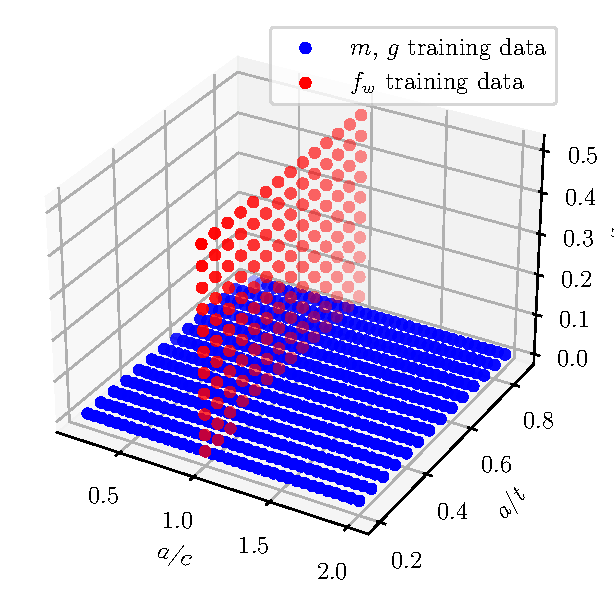
\includegraphics[width=\textwidth]{Figures_pdf/training_slices.pdf}
    \label{fig:training_models_3d}
    \caption{Visualization of the training data reduction allowed by the mechanics based approach. Each point represents a model in the training data-set. $f_w$ was trained when $\phi = \pi/2 \text{ and } a/c = 1$, $M$ was trained when $\phi=\pi/2 \text{ and } c/b = 0$, and $g$ was trained when $c/b = 0$ }
\end{figure}


During the training process, two techniques were employed to enhance the predictive ability and interpretability of the models. The first of these techniques involved the use of custom fitness functions to enforce the known constraints of each equation. These fitness functions assess the suitability of each candidate equation at the end of each training generation. The use of custom fitness functions ensures that all equations identified by the bingo algorithm adhere to the known limits of each equation, thereby improving interpretability. For instance, in equation \ref{eqn:fw_parameter_def}, as the values of $a/t$ and $c/b$ approach zero, the value of $f_w$ converges to 1. A fitness function that calculates the loss when this condition is met and assigns an infinite loss when it is not met enforces the equation's limits. Similar limit constraints apply to $M$ and $g$, such as $M(a/c = 1) = 1$ and $g(\phi = \pi/2) = 1$. The other method used to modify the training process was the addition of seed functions in the initial population. In the initial generation of the Bingo algorithm, a population of randomly generated equations is created. Using seeded equations allows the user to designate a fraction of these randomly generated equations as pre-set equations. This enables users to provide guidance to the algorithm. For example, upon visual examination of the training data for $g$, it was observed that $\left(1 - \sin\phi\right)^{a/t}$ appeared to fit the data well. Additional Bingo models were trained with this function seeded into the initial population. Other Bingo models were trained with only $1 - \sin\phi$ while other had no seeding at all. 


Training Bingo on the functions $f_w$ and $M$ was relatively fast only requiring 1-2 days due to the small training data-set, which only contained one data point per model when $\phi = \pi/2$. Additionally, these functions only required the discovery of relationships between two variables, namely, $c/b$ and $a/t$ for $f_w$, and $a/c$ and $a/t$ for $M$. However, training the function $g$ presented a different challenge due to the substantial increase in the number of data points as this function is now trained on every value of $\phi$ in each model. The Bingo algorithm tends to slow down as more data points are added. This results in a data-set comprising 300-400 data points per model, in contrast to the single data point per model for $f_w$ and $M$. To expedite the training of the $g$ function, two strategies were employed. The first involved down-sampling the $\phi$ data to reduce it to only 20 data points per model. The second strategy made use of a Bingo feature called the fitness predictor island (FPI). FPI aims to identify the optimal subset of the data that best represents the entire data-set. The size of this subset is determined by a hyper-parameter that specifies the fraction the subset. Even with theses two methods of reducing the number of data-points Bingo still took 5-7 days to train the $g$ models that did not contain $c/b$ and up to 13 days for the models that did contain $c/b$.


Once each training data-set has been computed bingo can be trained to find all three equations for $f_w$, $M$, and $g$ simultaneously. Multiple models were trained for each of the functions, due to the randomness of genetic programming this gave new equations that could be compared to one another to find the best combinations of $f_w$, $M$, and $g$ that predict SIF. The training process is done by first taking the SIF data computed from the FE model and then extracting the $f_w$, $M$, and $g$ training data-sets. Then bingo equations can be found for all three equations, these equation are then combined with the embedded ellipse solution from equation \ref{eqn:K_semi_with_l} to create a prediction for SIFS, this process is visualized in figure \ref{fig:training_flow}.

\begin{figure}
    \centering
    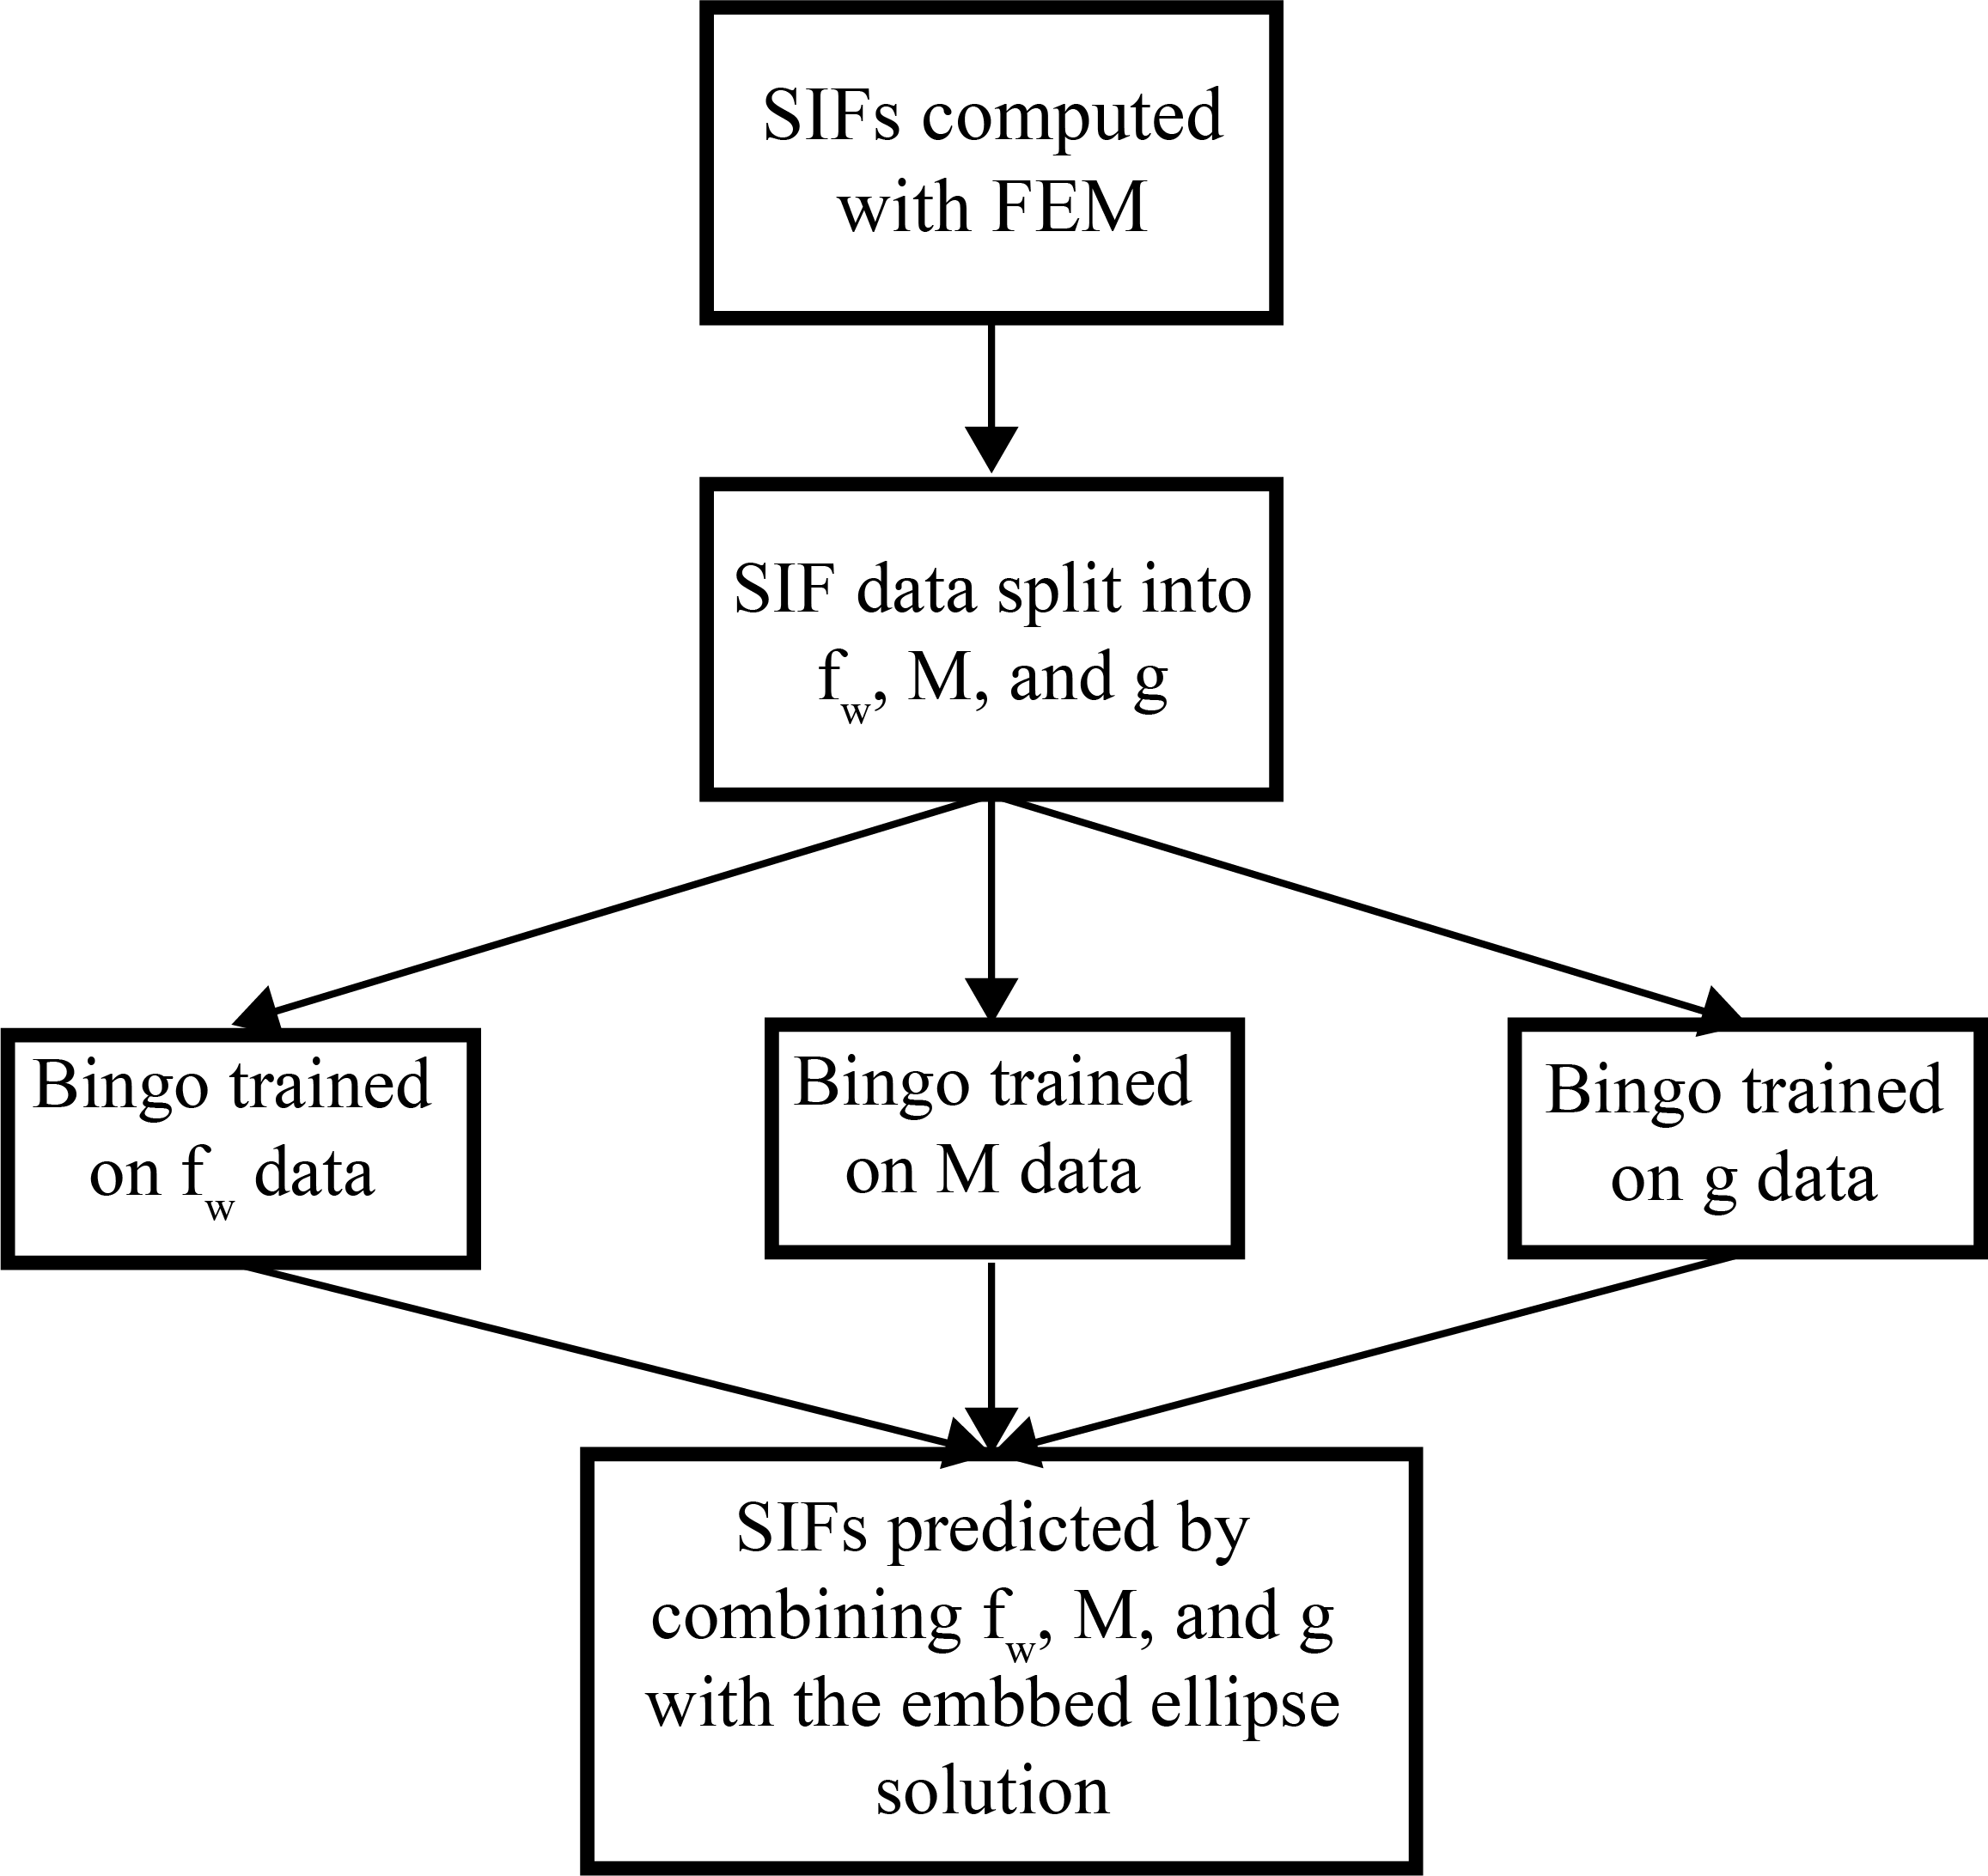
\includegraphics[width=\textwidth]{geometry_figures/training_flow.png}
    \label{fig:training_flow}
    \caption{Flow chart illustrating the training process of the three sub-functions $f_w$, $M$, and $g$}
\end{figure}




